\chapter{Introduction}

The diversity of physics programs at the LHC has made the analysis  in this thesis possible. Two consecutive datasets taken in late 2017---at \s = 5.02~\TeV and \s = 13~\TeV respectively---provide data with significantly lower pileup contributions than the standard conditions of Run II.  The unique configuration of these consecutive runs provides the opportunity to produce a set of measurements with high precision at two center-of-mass energies. 

This chapter provides a general overview of the physics and motivations for this measurement, as well as a brief description of the analysis strategy and what types of results will be produced. Chapter~\ref{ch:sm} provides a more detailed physics overview, Chapter~\ref{ch:exp} describes the LHC and CMS, and later chapters provided details of the individual components necessary for the measurement.


\section{A Brief Physics Background}

\subsubsection{Producing \W and \Z in \pp collisions}
Protons are composite particles consisting of quarks and gluons. The composition of protons can be described by the valence quarks, sea quarks, and gluons. The valence quarks of $p$ are two up quarks and one down quark ($uud$), which combine to make the color-neutral proton with +1 electric charge. The momentum distributions of the constituent quarks and gluons are described by parton distribution function, which have been determined through deep inelastic scattering experiments. At the high energies attained at the LHC, this internal structure within the protons being collided becomes extremely important to understanding the interactions occurring within the \pp collisions. \W and \Z bosons are produced through the Drell--Yan process, with the predominant production interactions: $u\bar{u}, d\bar{d}\rightarrow Z$,  $u\bar{d}\rightarrow W^+$,  and $d\bar{u}\rightarrow W^-$. In \pp collisions, these interactions therefore necessitate the participation of the sea quarks and predictions are sensitive to the sea quark PDFs. \phil{mention the prescence of anti-quarks motivates that you are probing the sea}.

\subsubsection{Electroweak Measurements}
Since the discovery of the \W and \Z bosons at UA1 and UA2 at CERN's Super Proton Synchrotron, their properties have been studied extensively at both hadron colliders and $e^+e^-$ colliders. The masses, branching fractions,  decay widths, and cross sections have been measured by multiple experiments, and some of these are known to high precision. Measurements of the \Z decay width at LEP provide constraints on the number of neutrino flavors. 
Past measurements of the W and Z boson cross sections at hadron colliders (Figure~\ref{fig:intro:summary:meas}) have been performed in \ppbar collisions at the UA1 \& UA2 experiments at the SPS, D\O ~and CDF experiments at Fermilab's Tevatron, and in \pp collisions by experiments at the LHC. 
Cross sections of \Wpm and Z boson production at the LHC has been studied at \s $= 2.76$, $5.02$, $7$, $8$, and $13$ \TeV by the CMS, ATLAS, and LHCb experiments~\cite{Aad:2019bdc,Aaboud:2018nic,Aaboud:2016btc,CMS:2011aa,Aaij:2014wba,Aaij:2012mda,Aaij:2015gna,Aaij:2016qqz,Aaij:2016mgv,Aaij:2015zlq,Chatrchyan:2014mua,Aad:2016naf}. \phil{mention where you result fits in}

\begin{figure}
\centering
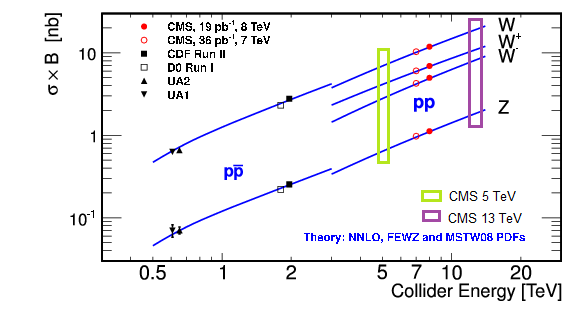
\includegraphics[width=0.6\linewidth]{plots/Intro/summary_v2.png}
%   \caption{1a}
%   \label{fig:Eff:el:5TeV:GSFSel:pos
\caption{Summary of previous measurements of the \W and \Z boson production cross section at hadron colliders. Not shown are the results from \sh LHC measurements. Measurements presented in this thesis are also indicated. Adapted from \cite{article_wzsummary}.}
\label{fig:intro:summary:meas}
\end{figure}

\section{Measuring the cross sections}
\subsubsection{\W and \Z decays}
\W and \Z bosons can decay both hadronically and leptonically. The leptonic decays \zee and \zmm provide extremely clean signatures marked by the presence of a pair of oppositely charged leptons. Similarly, the decay channels \wenu and \wmunu can be identified by the presence of a high-momentum electron or muon. Electrons and muons within CMS can be identified and reconstructed well, lending themselves to this measurement as a clean sample and accurately modeled observables are important to the success of a precision measurement.
\subsubsection{Cross section}
The cross section times branching ratio for a given channel is measured experimentally by determining the number of signal events observed and accounting for the acceptance of the measurement, as shown in Equation~\ref{eq:eq_xsec}. The acceptance of the fiducial volume is determined from simulation, and the efficiency scale factor is determined by measuring selection efficiency in both simulation and data. The following chapters of this thesis describe the derivation of these quantities in detail.
\begin{equation}\label{eq:eq_xsec}
\sigma\times Br = \frac{N_{signal}}{A\epsilon \int\mathcal{L} dt}
\end{equation}
\begin{itemize}
\item \nsig: Number of signal events observed in a given channel
\item $A$: The acceptance is the number of \W or \Z bosons producing a final state with leptons inside the fiducial measurement volume, divided by the total number of \W or \Z bosons produced. Determined from simulation. 
\item $\epsilon$: The efficiency scale factor, to account for the differences in rates of lepton identification and selection between simulation and data
\item $\int\mathcal{L}dt$: integrated luminosity. The integrated luminosity provides the number of $pp$ collisions measured in a given dataset.
\end{itemize}

\subsubsection{Z boson cross section}
Determining \nsig for the Z boson is fairly straightforward, as the dilepton decay of a Z is an extremely clean signature with minimal background. Two well-identified leptons are taken to be candidates for \zll decays, and events with invariant mass \masswindow are counted. Small background contributions primarily from diboson and \ttbar events are simulated, and the total contribution of the background processes is subtracted from the observed \zll yield. 



\subsubsection{W boson cross section}
The W decay channels used in this measurement include the production of a neutrino, which is not measured by CMS. Therefore, the final state cannot be fully reconstructed, and additionally has a fairly large background. Instead of a fully reconstructed final state, an observable, transverse missing energy, \met, is used to differentiate between the signal and background. The expected \met distribution for the \wlnu process, as well as several background processes, are used in a fit to data to extract the yield for \nsig as well as the background contributions. 
Measuring the W cross section relies heavily on the Z boson---there are multiple corrections that need to be derived for the W that cannot be done without the Z. In addition to the lepton efficiency and momentum corrections, the fit to \met requires an accurate modeling of hadronic recoil in an event. Hadronic recoil corrections account for differences between simulation and data, and are derived in a data-driven approach which relies on the Z boson, and are described in Chapter~\ref{ch:recoil}. 


\subsubsection{Measurements}
The results presented in this thesis are derived from datasets with \s = 5.02 \TeV and \s = 13 \TeV. This provides the opportunity to produce results with the highest precision available for two center-of-mass energies. The measurements are presented as the cross sections for \Wp, \Wm, \W, \Z, as well as the ratios of the cross sections $W^+/W^-$, $W^+/Z$, $W^-/Z$, $W/Z$. Evaluating the ratios allows the subtraction of any correlated systematic uncertainties, and increases the precision of the measurement. Notably, the uncertainty from the luminosity calibration is one of the largest uncertainties, and it completely cancels for these ratios. Additionally, making separate measurements at \s = 13 \TeV and \s = 5 \TeV provides another method for providing results with reduced uncertainties---taking ratios of the quantities: [13 \TeV]/[5 \TeV] allows us to further remove any correlated uncertainties. Some of the uncertainties which are correlated in this manner are the luminosity calibrations (partial correlation) and the theoretical uncertainties on the predictions. 

%% Where to put this section
% \section{\W and \Z bosons at the LHC}
% In proton-proton collisions, the primary mode of production for both the \W and \Z bosons is the Drell-Yann process. The valence quark composition of the protons is $uud$, so at least one sea quark is required for \W or \Z production. The processes are primarily $u\bar{u}, d\bar{d}\rightarrow Z$,  $u\bar{d}\rightarrow W^+$,  and $d\bar{u}\rightarrow W^-$. 

% The \W and \Z both decay via hadronic and leptonic channels, with branching fractions LOOK UP IN PDG. The leptonic decay channels have $Br(Z\rightarrow ee) = Br(Z\rightarrow \mu\mu) = Br(Z\rightarrow\tau\tau)$ due to lepton universality. 
% The decay channels \zll and \wlnu provide extremely clean signatures, as electrons and muons are well-measured in CMS. The channels that this measurement is performed on are \zee, \zmm, \wenu, and \wmunu. 

% \begin{figure}
% \centering
% \includegraphics[width=\linewidth]{ch01/plots/zprod_dy.png}
% %   \caption{1a}
% %   \label{fig:Eff:el:5\TeV:GSFSel:pos
% \caption{Drell-Yann production of Z bosons.}
% \label{fig:ch08:prefire:2017H}
% \end{figure}


\section{Impact of the Measurement}
\W and \Z boson production is an important measurement at any hadron collider. The precision measurement of the \W and \Z  production provides a precision test of the Standard Model as well as a benchmark for the state-of-the-art calculations and models that are used to describe the proton and simulate physical interactions at the LHC and other experiments. The inclusive cross section measurements are the foundation of differential cross section measurements which provide greater constraints on different aspects of the models.  \W and \Z production is also \phil{a} significant background to many other electroweak measurements and searches for new physics.
Additionally, \W and \Z bosons are a significant source of isolated, high-\pt leptons. The clean signature of \zll is used for detector calibration and luminosity monitoring \cite{xinmei}.
